\newpage
\section{Data visualization}

\section*{Outliers in the dataset}
The boxplot analyse method have been used for detecting outliers in the data set. 

\begin{figure}
\begin{tabular}{cc}
  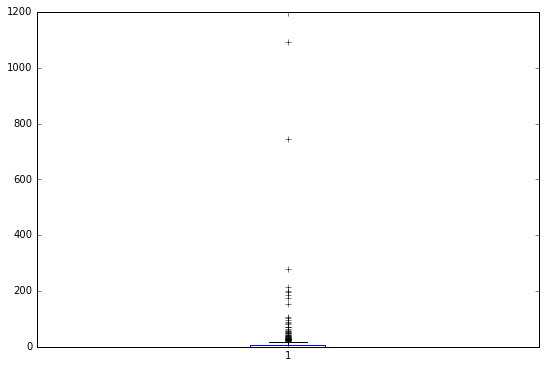
\includegraphics[width=65mm]{images/boxplots/area.png} &   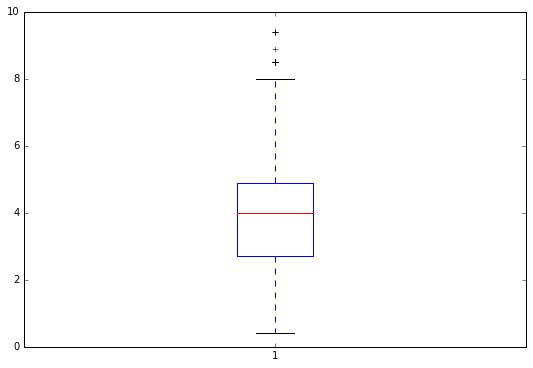
\includegraphics[width=65mm]{images/boxplots/wind.png} \\
(a) area & (b) wind \\[6pt]
 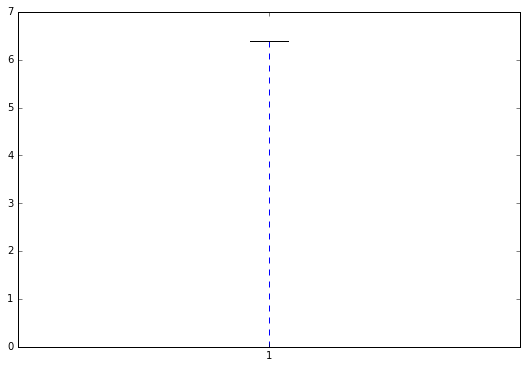
\includegraphics[width=65mm]{images/boxplots/rain.png} &   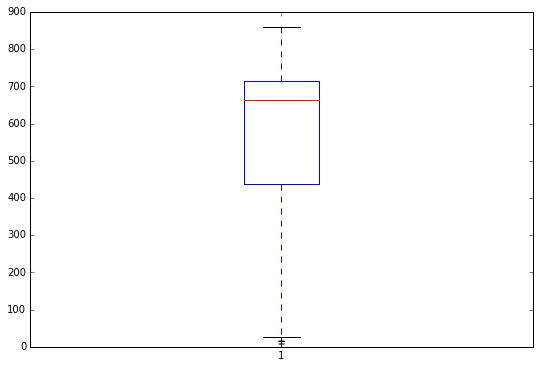
\includegraphics[width=65mm]{images/boxplots/DC.png} \\
(c) rain & (d) DC \\[6pt]
  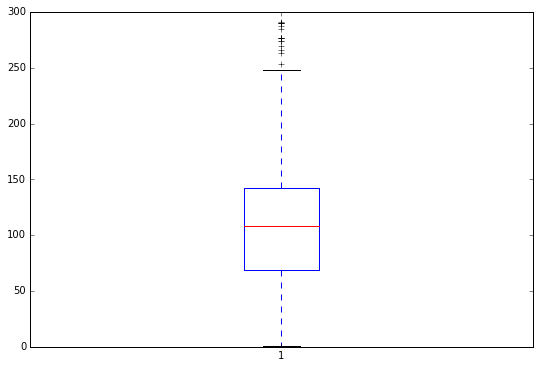
\includegraphics[width=65mm]{images/boxplots/DMC.png} &   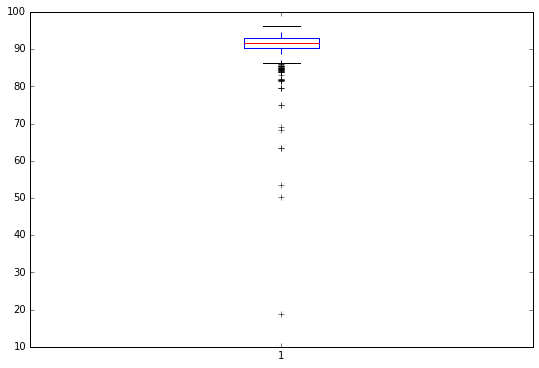
\includegraphics[width=65mm]{images/boxplots/FFMC.png} \\
(a) DMC & (b) FFMC \\[6pt]
\end{tabular}
\caption{Boxplot diagrams}
\end{figure}

\newpage

\begin{figure}
\begin{tabular}{cc}
 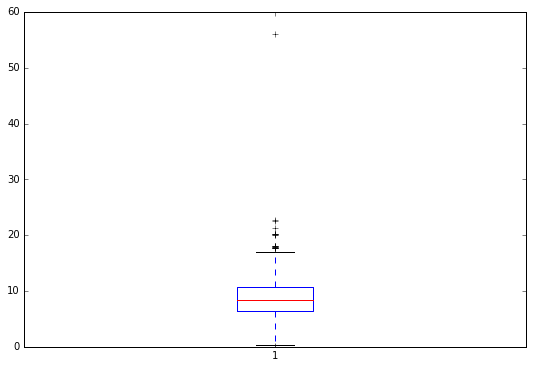
\includegraphics[width=65mm]{images/boxplots/ISI.png} &   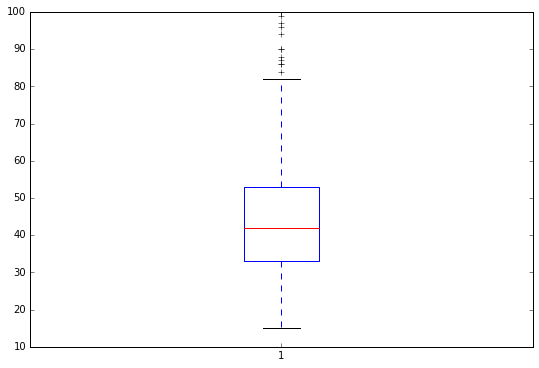
\includegraphics[width=65mm]{images/boxplots/RH.png} \\
(c) ISI & (d) RH \\[6pt]
  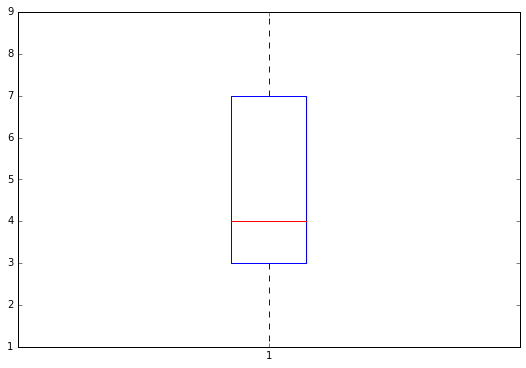
\includegraphics[width=65mm]{images/boxplots/x.png} &   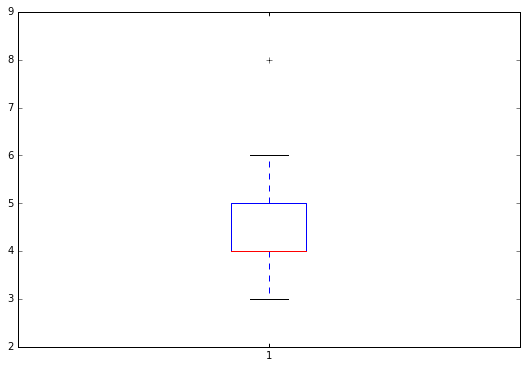
\includegraphics[width=65mm]{images/boxplots/y.png} \\
(a) X & (b) Y \\[6pt]
\multicolumn{2}{c}{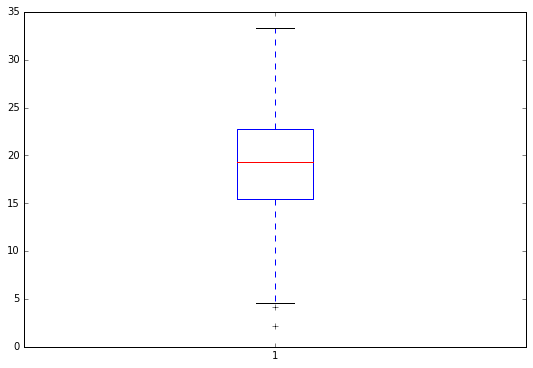
\includegraphics[width=65mm]{images/boxplots/temp.png} }\\
\multicolumn{2}{c}{(e) temp}
\end{tabular}
\caption{Boxplot diagrams}
\end{figure}